\scanpage{97}
% archive sheet number: 99

expliciter le lien du paramètre $a$ avec le paramètre $\tau$, ou mieux, avec l'invariant modulaire $j\in\mathbb R^{\unsure{*|?|\pm}}$ (serait-on $j=\unsure{\pm|4|\tfrac12}\log a$ ?) \deleted{i.e. $a=\exp j$ ou $a=\exp -j$, suivant qu'on est dans la famille $E_a$ ou $E'_a$ ?)}.

\figure{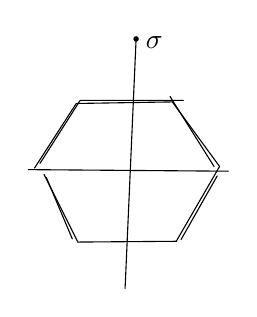
\begin{tikzpicture}[line cap=round]
\draw (0,0)--(.53,.82)--(1.75,.84)--(2.35,.02)--(1.80,-.93)--(.55,-.94)--(.12,-.08);
\draw (.07,.06)--(.58,.86)--(1.89,.86) (1.72,.91)--(2.28,.02) (1.86,-.91)--(2.32,-.10) (.15,-.12)--(.48,-.90);
\draw (-.08,-.02)--(2.46,-.04) (1.15,-1.53)--(1.29,1.64);\fill (1.29,1.64) circle[radius=.035];\node[right] at (1.29,1.59) {$\sigma$};
\end{tikzpicture}}

\deleted{Considérons} Notons que si $\sigma$ est dans $G^-$ alors \inserted{(réflexion par r. à \unsure{un relèvement|une droite} \unsure{orthogonal à celui|orthogonale à celle|hexagonal} de $\sigma$)} suivant les cas $-\sigma$ est conjugué, ou non conjugué, à $\sigma$. Dans le cas hexagonal, il est non conjugué, dans le cas carré, il est conjugué. Dans les cas non extraordinaires, $n=2$, il est bien sûr non conjugué (car $G$ est alors commutatif) --- donc le cas \deleted{hexagonal} \inserted{carré} est le seul où $-\sigma$ \deleted{\unsure{ne|n'}} soit \deleted{\unsure{pas}} conjugué à $\sigma$. \deleted{Donc sauf dans le cas carré peut-être, on trouve}

\uline{Distinguons les cas}

1) \uline{$n=2$} Cas non extraordinaires. Le groupe des autom est $\pm1,\pm\sigma$, où $\sigma$ est un \inserted{anti} autom. On voit de suite que si $\sigma$ est du type somme directe d'un $\mathrm{id}_P$ et $-\mathrm{id}_Q$, il en est de $=$ de $-\sigma$ (avec $P,Q$ échangés) donc on est dans cas $E_a$, ou \deleted{\unsure{$Q$|$a$}} \inserted{${}^a$} dans cas $E_a$ et un $E_{a'}$, correspondant aux deux éléments de $\unsure{\sigma|\sigma,},\sigma'$ de $G^-$, et on aura $aa'=1$. \deleted{\unsure{En|Enf}} en prenant un génér. \inserted{$u=$}$e_+$ de $\unsure{\pi_+|\Gamma_+|\Pi_+}$, un autre, \inserted{$v=e_-$} de $\pi_-$, on a

\[
a=a(\sigma)=\frac{Q(e_-)}{Q(e_+)}
\]

et comme par passage de $\sigma$ à $-\sigma$ \deleted{les} $e_+$ et $e_-$ s'interchangent, on aura bien

\margin{Ceci vaut aussi bien dans les cas des $E_a$, que des $E'_a$}

\[
a(-\sigma)=1/a(\sigma)
\]

(valable dans tous les cas), donc

\[
a(-\sigma)=a(\sigma)\Longleftrightarrow a(\sigma)=1\Longleftrightarrow\text{Cas \uline{carré}}.
\]
